\newpage

\section{Pulse Width Modulation (PWM), Servo Calibration (pulse =
  f(angle)) and Feedback Control}
\label{s:pwm}

\subsection{Parts List}

\begin{enumerate}[itemsep=-5pt]
\item CPX/CPB
\item USB Cable
\item Laptop
\item protractor or piece of paper
\item servo
\item Alligator clips (x3)
\end{enumerate}

\subsection{Learning Objectives}
\begin{enumerate}[itemsep=-5pt]
\item Understand what a PWM signal is and how it affects a servo
\item Understand the inner workings of a servo and how to make it move
\item Practice first order regression and calibration techniques
\item Understand how to compute roll and pitch from an accelerometer
\item Learn the fundamental concepts of feedback control
\item Learn how to Combine two codes (servo code and accelerometer code into one)
\end{enumerate}

\subsection{Getting Started}

For this lab we are going to learn how to drive a \href{https://www.adafruit.com/product/1143}{servo}. Servos accept what are called PWM signals which are basically square waves of varying frequency. The servo itself has a microprocessor on board that turns a DC motor based on the incoming PWM frequency which is typically called a duty cycle. The DC motor runs through some gear to rotate a shaft. Because of this rotation, you can make a number of things move! Servos are used for all sorts of things, opening doors, deflecting control surfaces on RC aircraft and many more! The neat thing about PWM signals is that they can not only move servos but they can also drive speed controllers to turn 3 phase motors and even change the light intensity of LEDs. Servos typically come in two different color schemes as shown below.
\begin{figure}[H]
  \begin{center}
    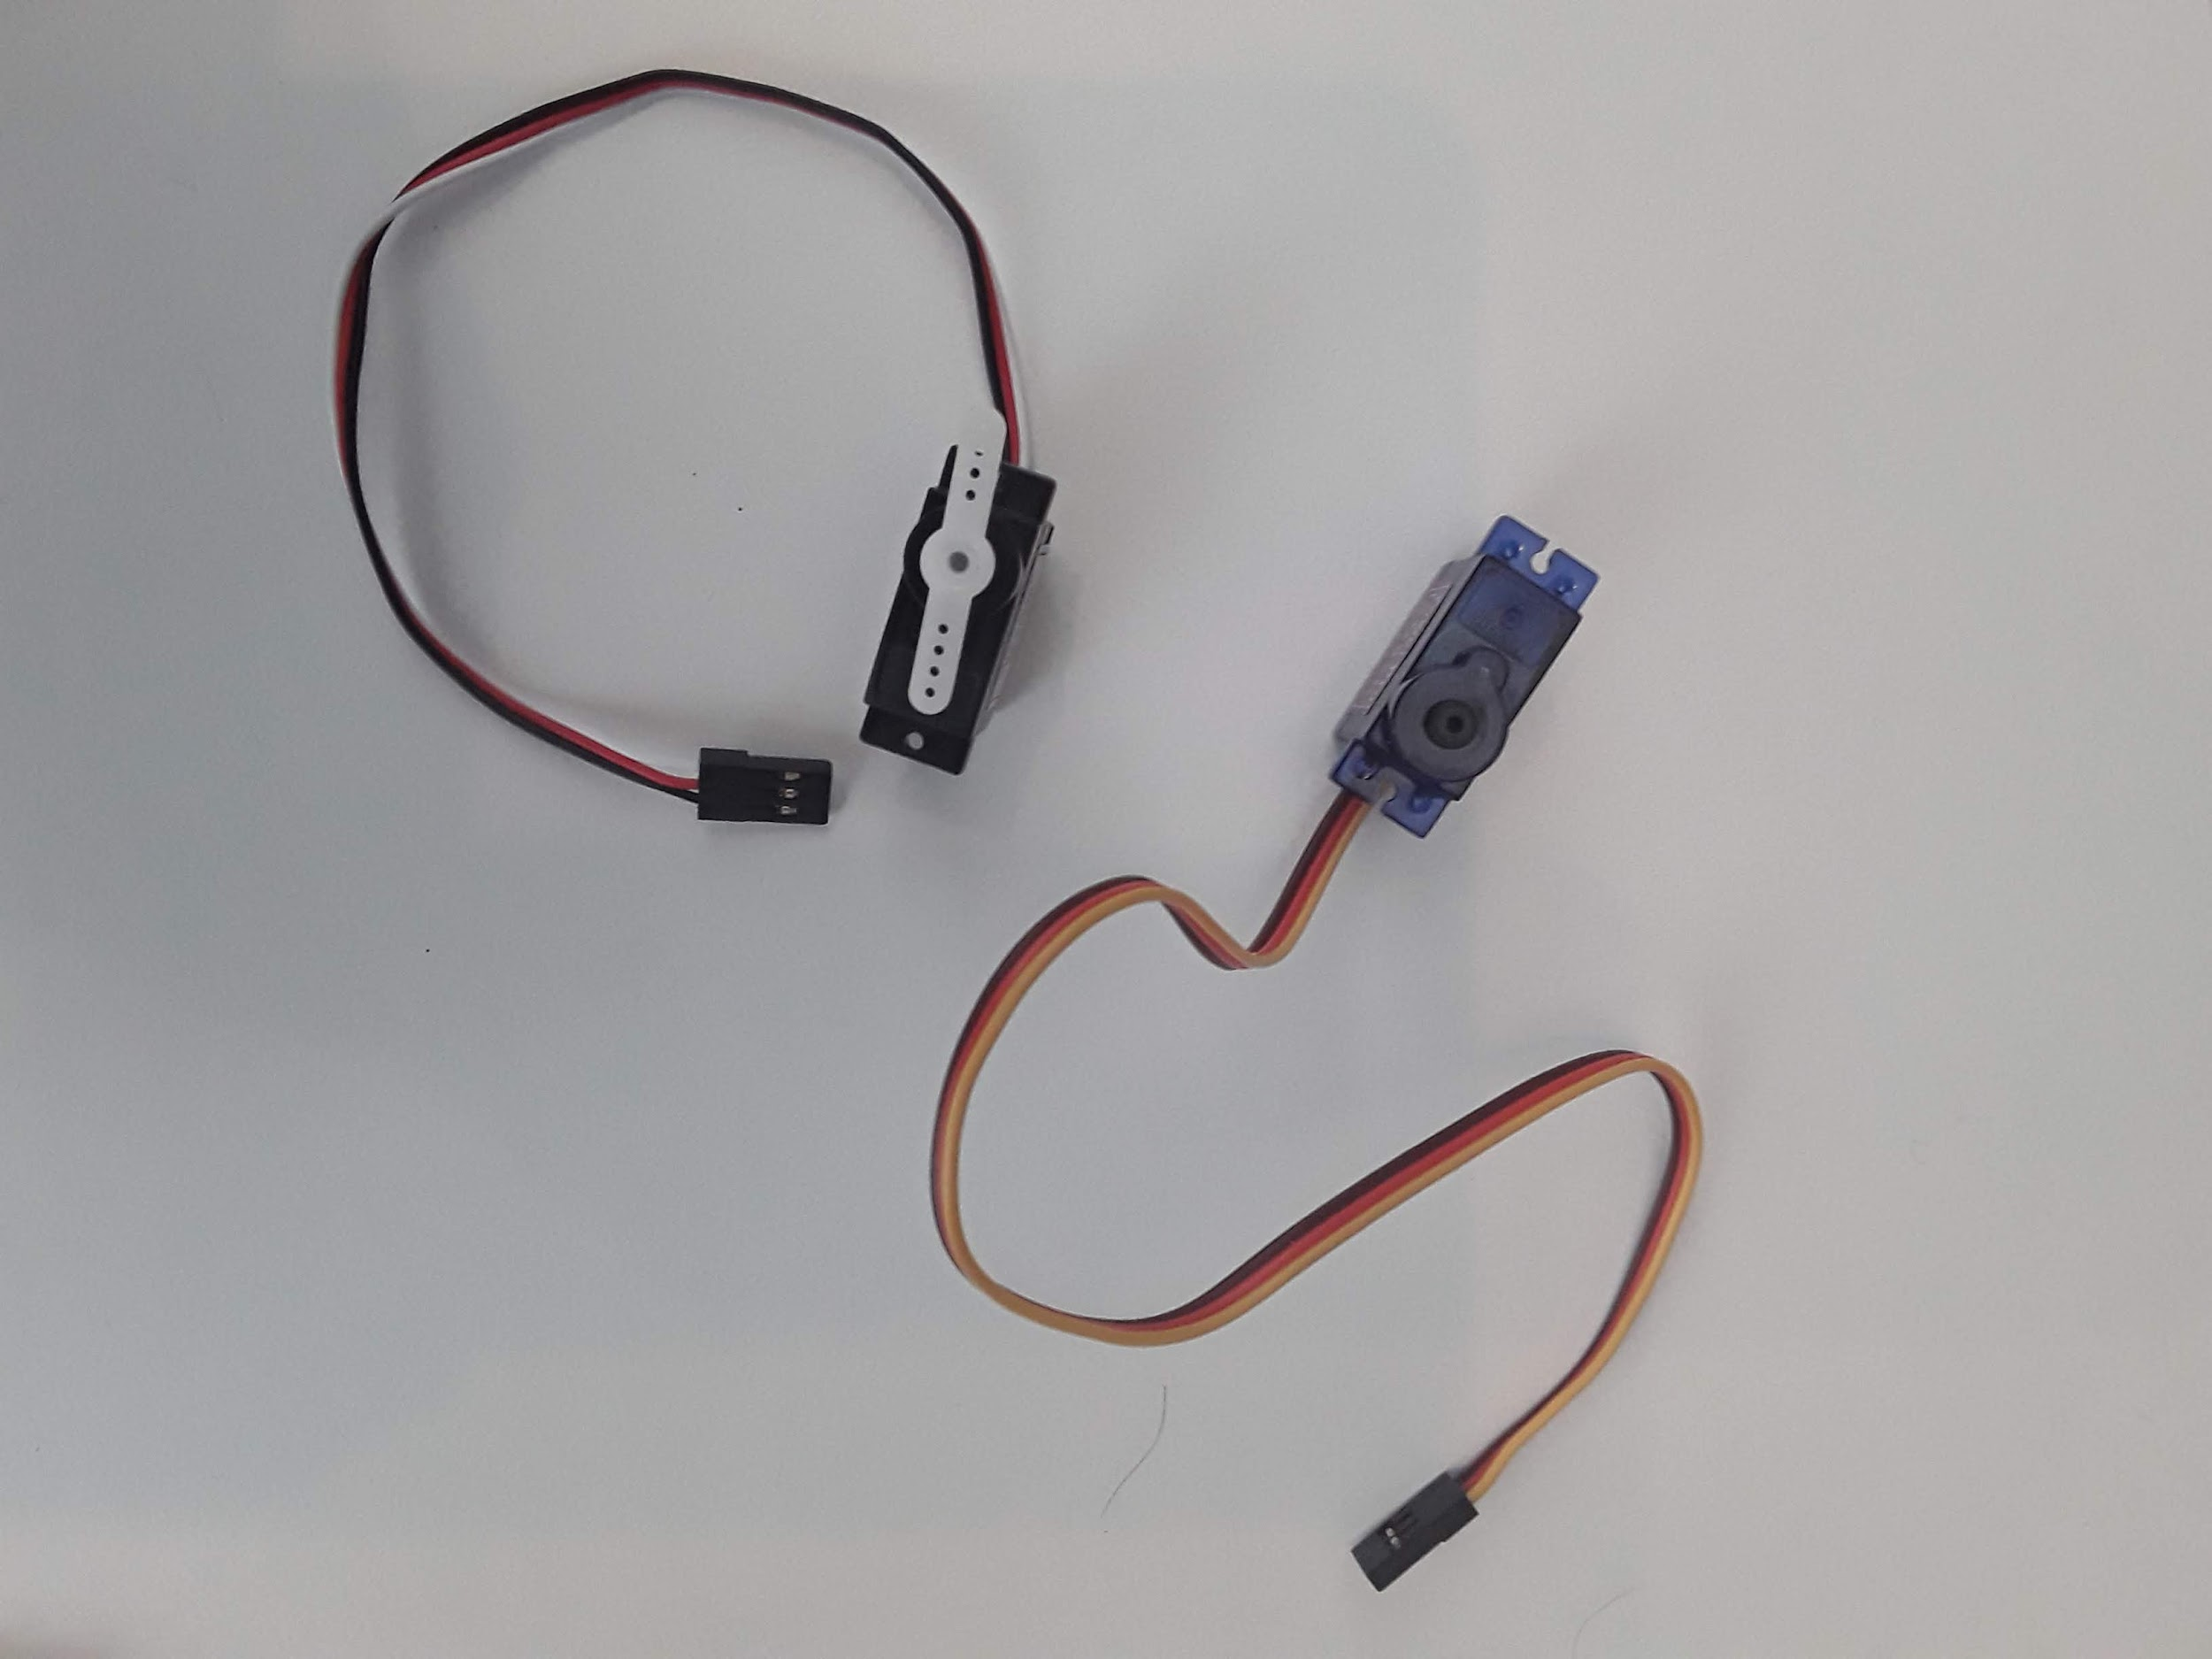
\includegraphics[width=0.8\textwidth]{Figures/servo.jpeg}
  \end{center}
\end{figure}
As you can see, servos have 3 pins - the brown or black wire is GND, the red wire needs to go to a 5V signal so for the CPX it needs to go to the VOUT pin and the yellow or white wire is the signal wire which need to go to an analog port on the CPX that supports PWM signals. Which ones support PWM signals? \href{https://learn.adafruit.com/adafruit-circuit-playground-express/pinouts}{Adafruit Learn} has a great description of which pins support PWM signals but as a quick check you can use the following analog pins: A1, A2, A3, A6 and A7. In my circuit I just picked pin A2 since I’ve been using it so much in the past.
\begin{figure}[H]
  \begin{center}
    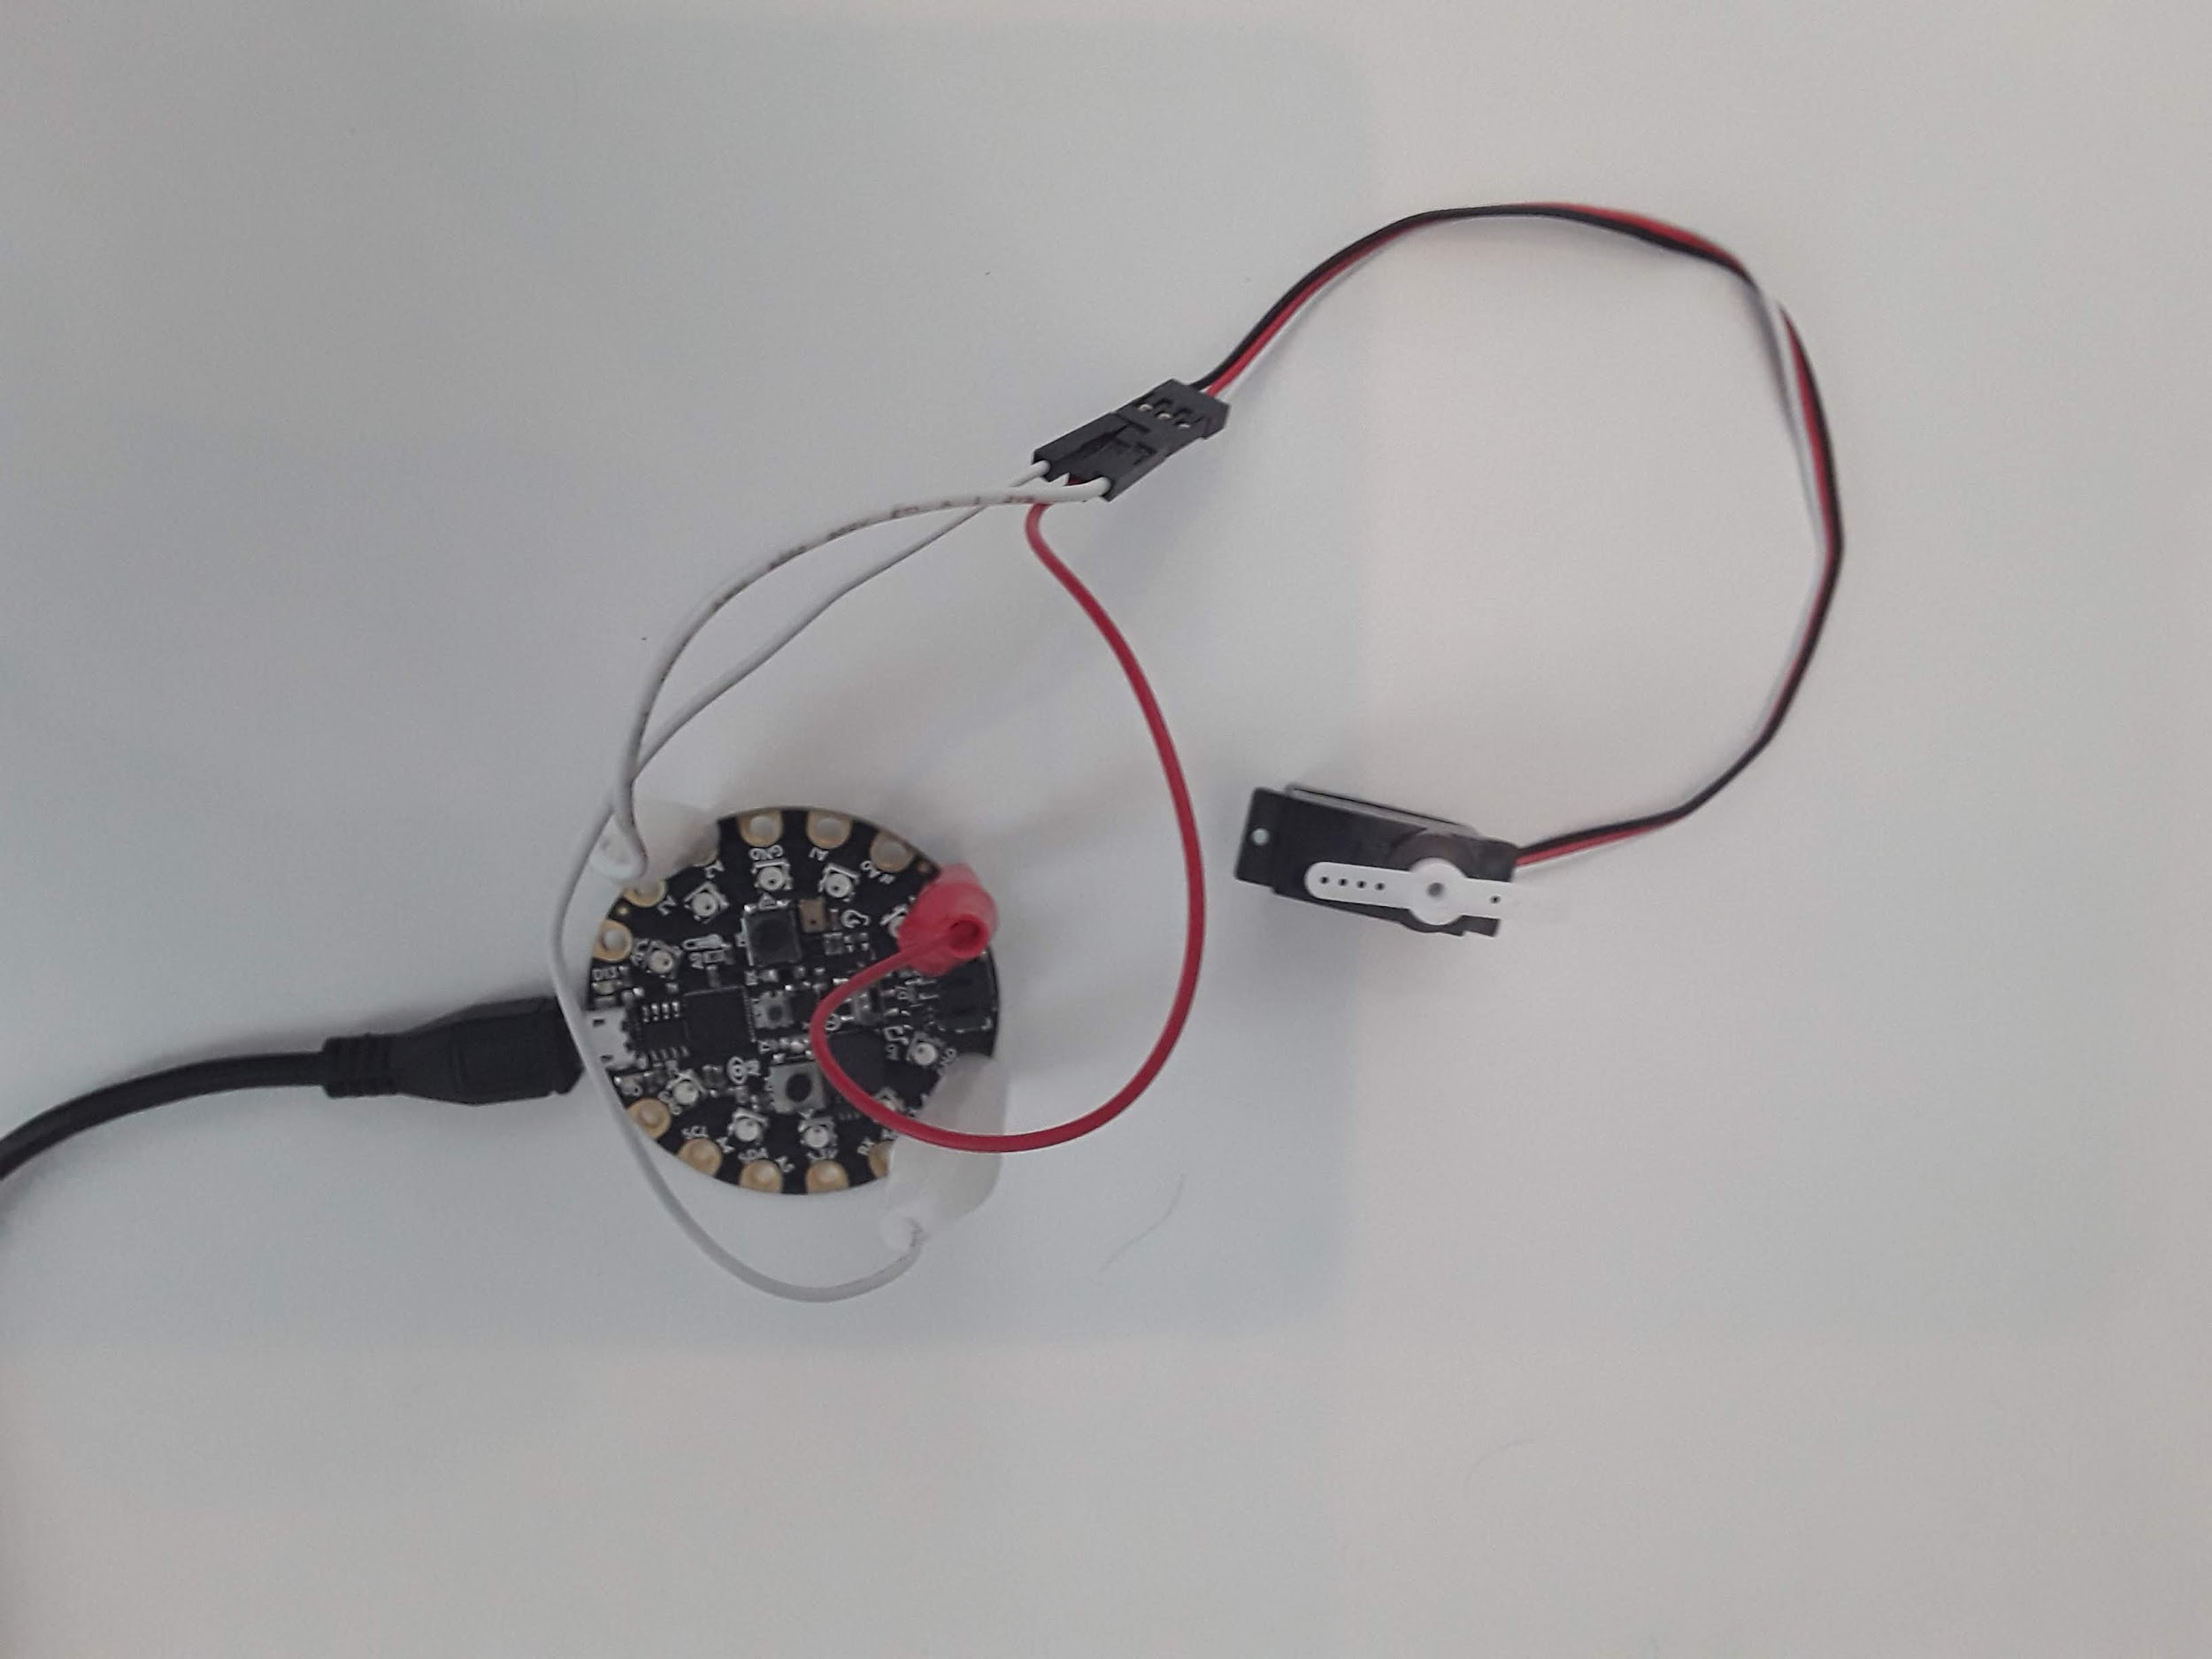
\includegraphics[width=0.8\textwidth]{Figures/servo_circuit.jpeg}
  \end{center}
\end{figure}
{\bf Very important: It is recommended to power a servo through an external power supply instead of the CPX. Servos can draw a lot of current and the CPX although it supports 5V can only provide so much power (P). Remember that P = VI so if P is low it means current is low. If the servo pulls more current than the CPX can provide the CPX will “brown out” which means it will go into a safe-mode setting. If you have the AA power supply you may consider doing that. For small servos you hopefully won’t have any issues.}

    As I said before, a servo takes in a square wave. The square wave has a duty cycle in units of microseconds. If you send a roughly 500 us square wave to a servo it will rotate all the way to the left. If you send a roughly 2500 us signal to the servo, it will turn all the way to the right. The code to send PWM signals has been thoroughly explained in the \href{https://learn.adafruit.com/using-servos-with-circuitpython/overview}{Adafruit Learn system}. I also have a \href{https://github.com/cmontalvo251/Microcontrollers/blob/master/Circuit_Playground/CircuitPython/Servo/servo.py}{simple servo.py script} on Github. In this code as usual the top 3 lines are used to import the necessary modules. The pulseio module is used here to create a servo object on line 6 by connecting to pin A2. Make sure to change the pin to whatever pin you have the signal wire hooked up to. Lines 9-12 create a function that pulse in milliseconds and compute the duty cycle of PWM signal. Lines 16-19 then kick off an infinite while loop where a 800 us signal is sent to the servo and then a 2000 us signal is sent using a for loop which starts on line 16. You’ll see servo command on line 18 which is responsible for sending the microsecond signal to the servo. The function servo\_duty\_cycle converts the pulse in milliseconds to a duty cycle. The value is then passed to the attribute of the servo object servo.duty\_cycle. If you put this code on the CPX and run the code you will hopefully see your servo turning left and right in 1 second intervals. I did this project myself and \href{https://youtu.be/ynlGiPZk5VM}{posted a YouTube video about it}. 

Besides making the servo move back and forth I’d like you to vary the pulses on line 16 {\bf SLOWLY} until the servo can’t move any farther. This line of code is a for loop which loops through the array currently showing [0.8,2.0]. If you change that array to [0.9,1.2,1.5,1.8] the servo will move to a pulse in milliseconds of 0.9, 1.2, 1.5 and then 1.8. The for loop is a great way to loop through multiple commands. Using this array, determine the minimum pulse you can send to the servo and the maximum pulse you can send to the servo. If the servo makes a funny noise it means you sent a signal outside the bounds so try a different signal. Hence the need for moving the pulse signal slowly. If you change the array to just 1 number [0.8] the servo will just move to 1 angle and stay there forever. {\bf NOTE THAT IN CIRCUITPYTHON VERSION 7.0.0 YOU HAVE TO USE THE PWMIO LIBRARY INSTEAD OF THE PULSEIO LIBRARY}.
\begin{figure}[H]
  \begin{center}
    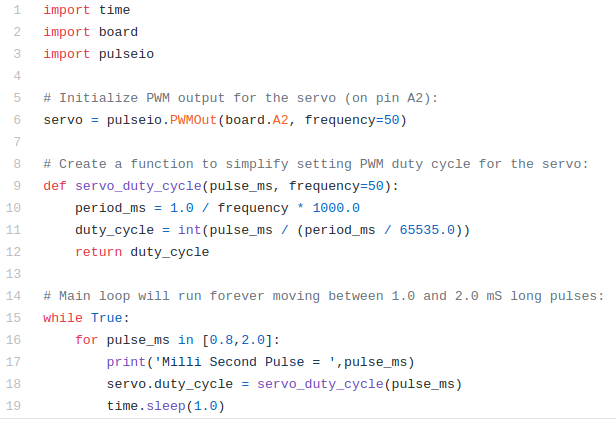
\includegraphics[width=0.8\textwidth]{Figures/servo_code.png}
  \end{center}
\end{figure}
If you notice, sending a pulse signal in microseconds moved the servo to a specific angle. Thing is I would like to be able to move the servo to a specific angle rather than having to just guess and check like we did in the last lab. So what we’re going to do is start at the minimum pulse signal you computed in the last project and then change the servo pulse in equal increments until we reach the maximum servo pulse signal. When I did this lab I found that 0.6 ms was just about the smallest I could get the servo to move. We’re going to call this 0 degrees. My maximum pulse signal ended up being about 2.4 ms. So I want you to test 10 different points between your specific maximum and minimum value which will hopefully be different for all of you. Everytime you test a pulse I want to measure the angle the servo makes with the minimum value being 0 degrees. Create a table of data with two columns. In the first column put pulse in milliseconds and in the second column put angle of servo in degrees. Use a protractor to measure the angle. \href{https://www.youtube.com/watch?v=XSLzcwTOsWk}{If you don’t have a protractor make one} or you can download a picture and hold your servo up to the screen. I did this project with just 3 data points and here are my data points. Again you need to have around 10 data points
\begin{table}[H]
\begin{center}
\begin{tabular}{|c|c|}
\hline
Pulse (ms) & Angle (Degrees) \\
\hline
0.6 & 0 \\
\hline
1.5 & 90 \\
\hline
2.4 & 180 \\
\hline
\end{tabular}
\end{center}
\end{table}
    Take your table of data and put it into a spreadsheet and save the data as a CSV or simply put your data into a text file. Since I only had 3 data points I just put them into a text file. Plot the data in Python on your desktop computer with servo angle on the x-axis and duty cycle on the y axis. Using the data, determine if the data set is linear, quadratic or cubic. Fit a trend line to the data and plot your trend line on top of the data. \href{https://www.youtube.com/watch?v=4vYYPHRMdqM&feature=youtu.be}{If you need help with trend lines in Python you can watch this video I posted on Youtube}. I also made a helpful \href{https://github.com/cmontalvo251/Python/blob/master/instrumentation/book_problems/least_squares_regression.py}{python script with some fictitious data on Github} that fits the data with linear and quadratic fits. Here is my data plotted alongside the trendline in Python. I sort of made up the data and made it perfect on purpose so my trendline is perfect. Yours will not be so perfect.
\begin{figure}[H]
  \begin{center}
    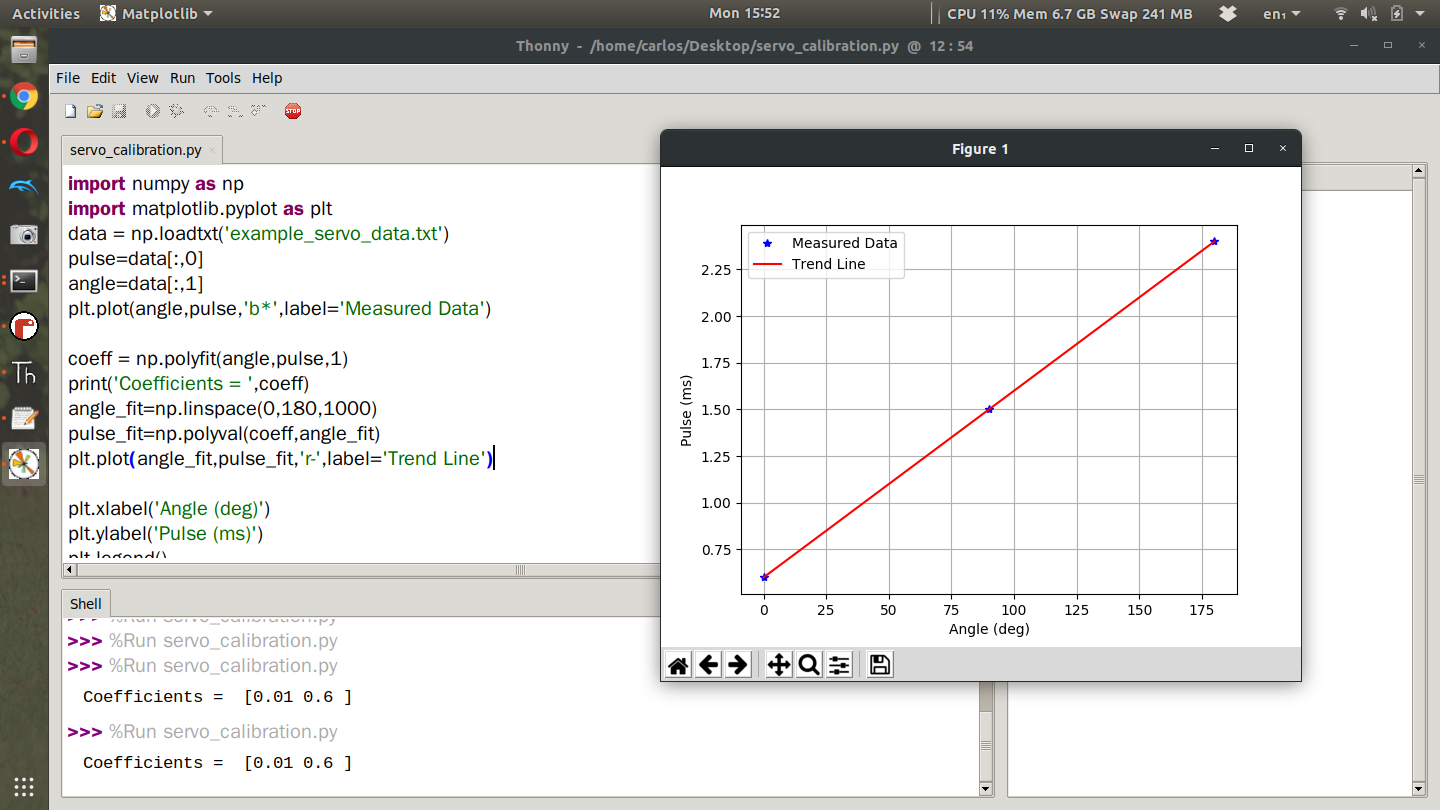
\includegraphics[width=0.8\textwidth]{Figures/trendline.png}
  \end{center}
\end{figure}
You’ll notice that I first import the data from the text file using the np.loadtxt function and then I use the polyfit and polyval functions to create the trendline. The polyfit function requires you to give it the X and Y axes and the order of the trendline which since the trend line is linear I sent it a 1 but you could easily do 2 for quadratic or 3 for cubic. I then print the coefficients which are [0.01 0.6]. This means my trend line looks like this.
\begin{equation}
Pulse = 0.6 + 0.01*Angle
\end{equation}
Where Pulse is in ms and Angle is in degrees. Now you have an equation where you can use angle in degrees to compute the pulse in milliseconds. In the code I’ve posted I then use np.linspace to create 1000 data points from 0 to 180 degrees and then use the polyval function to compute the pulse for all 1000 angles I created using the linspace command. I finally plot the trend line in red and use the remaining part of the script to create labels and legends. Once you have this plot write down your coefficients and create an equation like I did above. Again your numbers won’t be so neat. Once you have this equation, return to Mu and create a function using the def keyword that takes in an angle as an input and then returns a pulse signal in milli seconds. It will look sometime like this
\begin{verbatim}
def angle2pulse(angle):
        return 0.6 + 0.01*angle
\end{verbatim}
{\bf Note: Functions in python must be after all your imports but before your while loop. If you put this function inside your while loop the code will not work}. Using that equation, modify your servo.py script to have the servo move through the following angles, 0, 45,90,135 (your servo may not travel to 180 degrees). Verify that your equation is working correctly by placing your protractor below the servo. Much of the code required for this project is not included because it is left as an exercise for the student.

\subsection{Feedback Control}

Feedback control can be its own course or multiple courses but can be
broken down into a few simple steps. The goal of feedback control is
to drive the “state” of a “system” to a desired “command” by sending a
“control” signal to the “system”. I explain this in much more detail
in a
\href{https://www.youtube.com/watch?v=PAK5V8wzVXY&list=PL_D7_GvGz-v30U58EUUOdJGgO4u75DXoB&index=1}{controls
  overview Youtube video}. For this lab we are going to make the bare
bones circuitry required for pitch angle control of an airplane. The
“system” then is the aircraft. The “state” is the “pitch” angle
(measured by the CPX), the “command” is the desired pitch angle
(programmed by you the pilot in command) and the “control” signal is
the elevator command (actuated by a servo). I’m using the same circuit
I created in parts 1 and 2.

The elevator on an airplane is a control surface responsible for
pitching the aircraft up and down. For this example we are going to
assume that the desired pitch angle is 0. This means our “error”
signal is going to be 0 minus the pitch angle. Our “control” signal
will be the angle of the elevator. As I said, we are going to use a
servo to control the elevator so this just means we need a way to
relate our “error” signal to servo pulse width. There are a few steps
here before we can move on. First, we need to relate our “error”
signal to the “control” signal which will be the elevator pitch
angle. I’ve made a table below to explain what I mean. 
\begin{table}[H]
\begin{center}
\begin{tabular}{|c|c|c|}
\hline
Pitch (deg) & Error (deg) & Elevator (deg) \\
\hline
-90 & 90 & +90 \\
\hline
0 & 0 & -90 \\
\hline
+90 & -90 & -90 \\
\hline
\end{tabular}
\end{center}
\end{table}
This table basically says that if the aircraft is level with a pitch angle of zero I want the elevator to be zero as well. If the aircraft pitches down, I want the elevator to pitch up and counteract that rotation. Using these three data points I can create a simple equation to relate elevator angle to pitch angle.
\begin{equation}
\delta_e = -\theta
\end{equation}
Now that we have the elevator pitch angle we need to relate this to the servo angle. Servo can only move from 0 to 180 degrees which means we can’t have the servo go negative. Thus we need to offset the elevator angle to the servo angle. Again we can make a table here.
\begin{table}[H]
\begin{center}
\begin{tabular}{|c|c|}
\hline
Elevator (deg) & Servo (deg)\\
\hline
-90 & 0 \\
\hline
0 & 90 \\
\hline
+90 & 180 \\
\hline
\end{tabular}
\end{center}
\end{table}
This also results in a simple equation to relate servo angle to elevator angle.
\begin{equation}
s = \delta_e + 90
\end{equation}
Finally, we can then use our calibration coefficients (See chapter \ref{s:pwm}) to relate servo angle to pulse width. When I calibrated my servo I obtained the following equation where P is the pulse and s is the servo angle.
\begin{equation}
Pulse = 0.6 + 0.01*Angle
\end{equation}
With these 3 equations I can now program my servo to respond to changes in the pitch angle of the CPX. I did forget one minor detail and that is measuring the pitch angle itself. This is similar to measuring the angle of a pendulum (See chapter \ref{s:pendulum}). I’m going to rotate the CPX in the X/Z plane which can be done by rotating the USB cable where it plugs into the CPX. In this case we can ignore the Y axis data. If you print the raw accelerometer data, you’ll notice that when you place the CPX directly onto a flat surface, the x and y axes read a value around 0, while the z axis reads around gravity. If you then rotate the sensor clockwise 90 degrees, the x axis is reading about gravity while the z axis is now zero. This means we can form a triangle and get the angle using these two axes using the equation below which gives angle in degrees.
\begin{equation}
\theta = tan^{-1}(x/y)\frac{180}{\pi}
\end{equation}
On the CPX specifically we want to import the math module and use the atan2 function. With this equation I can finally put it all together. Here is my code which again is also \href{https://github.com/cmontalvo251/Microcontrollers/blob/master/Circuit_Playground/CircuitPython/Servo/feedback_control_servo.py}{online on Github}.
\begin{figure}[H]
  \begin{center}
    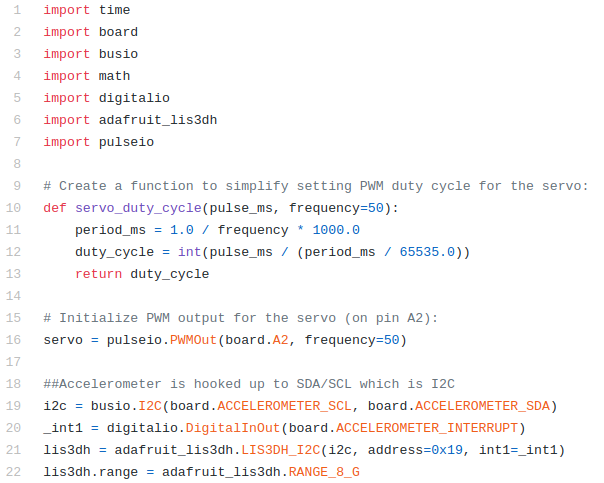
\includegraphics[width=0.8\textwidth]{Figures/feedback1.png}
  \end{center}
\end{figure}
The first 22 lines here will hopefully seem familiar. Line 1-7 are import commands of all the various modules needed. Lines 10-13 create the definition that converts pulse width to duty cycle. Line 16 creates the servo and lines 19-22 create the accelerometer. Hopefully this is a good example of combining different codes together to get a more complex piece of software. Lines 24-45 include a very long while loop. I will try and go through each line. Line 26 grabs the accelerometer data on the CPX. Line 28 uses the x and z axis accelerometer data and converts the values to pitch angle using the atan2 function in the math module which was imported on line 4. Line 30 computes the elevator pitch angle and line 32 computes the servo deflection angle. Line 34-37 is a type of signal conditioner called a saturation filter. Basically, I don’t want the servo to break because I tried to make the servo rotate more than 180 degrees or less than 0 degrees. So I created two if statements that restrict the servo to be within these two values. If the servo angle is less than 0 as stated on line 34, the servo angle is set to 0 on line 35. If the servo angle is greater than 180 as stated in line 36 the servo angle is set to 180.
\begin{figure}[H]
  \begin{center}
    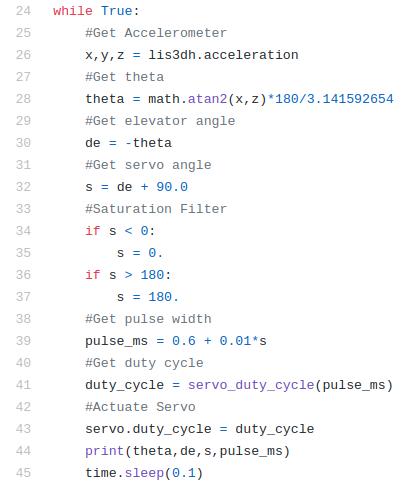
\includegraphics[width=0.6\textwidth]{Figures/feedback2.png}
  \end{center}
\end{figure}
Line 39 uses the calibration equation from the previous experiment to convert servo angle to pulse width. You’ll need to replace these numbers with your servo since all servos are different. Line 41 uses the definition created on lines 10-13 to convert pulse width to duty cycle. Line 43 makes the servo move. Line 44 prints everything to Serial for debugging purposes and line 45 pauses the script for 0.1 seconds which helps with some twitchiness in the servo. When I did this I didn’t have to program a complementary filter so I guess the servo may have it’s own low pass filter. Either way this circuit is ready to be placed on an aircraft. Whether or not it is effective is a completely different story. I’ll leave that discussion to your controls professor. Note you can also include the angular rate sensor and use that as derivative gain as well.

\subsection{Assignment}

Upload a PDF with all of the photos and text below included. My recommendation is for you to create a Word document and insert all the photos and text into the document. Then export the Word document to a PDF. For videos I suggest uploading the videos to Google Drive, turn on link sharing and include a link in your PDF.
\subsubsection{Part 1}
\begin{enumerate}[itemsep=-5pt]
\item Send a video of your servo moving back and forth (make sure your face is in the video and make sure you introduce yourself) - 50\%
\item Experimentally determine the minimum and maximum values of the servo and report the 2 PWM signals in milliSeconds. Give at least 2 decimal points in your calculation - 50\%
\end{enumerate}
\subsubsection{Part 2}
\begin{enumerate}[itemsep=-5pt]
\item Submit a video of you explaining how you took calibration data (make sure you are in the video and you introduce yourself) - 25\%
\item Include a Figure of your your data plotted in Python with your trend line on top - 25\%
\item Write your regression equation as servo\_pulse = m*servo\_angle + b - 25\%
\item Submit a video of your servo moving through 0,45,90,135 using the output from your regression equation. The regression equation must be placed into your while True loop rather than computed ahead of time -  25\% 
\end{enumerate}
\subsubsection{Part 3}
\begin{enumerate}[itemsep=-5pt]
\item Explain your circuit and what wires go where as well as all the parts of the feedback control system starting with the accelerometer. Only spend a minute or less explaining this - 10\%
\item Explain your code at a high level. Only spend a minute or less on how it works - 20\%
\item Show your servo moving as you rotate the CPX - 50\%
\item Verify that your saturation filter works correctly by rotating your CPX past 90 degrees (You may need to increase the sensitivity of the servo depending on your feedback control law) - 20\% 
\end{enumerate}
